\setcounter{section}{2}
\section{LPC17xx System control}

\subsection{Resumen del bloque}
\begin{itemize}
  \item Reune funciones globales del microcontrolador que no pertenecen a un perif\'erico puntual.
  \item El cap\'itulo concentra cuatro \'areas: \textbf{reset}, \textbf{brown-out detection}, \textbf{interrupciones externas} y \textbf{flags/controles de sistema}.
  \item Los registros clave del bloque son \texttt{EXTINT}, \texttt{EXTMODE}, \texttt{EXTPOLAR}, \texttt{RSID} y \texttt{SCS}.
\end{itemize}

\subsection{Pines asociados}
\begin{table}[H]
  \centering
  \small
  \renewcommand{\arraystretch}{1.15}
  \caption{Pines asociados al bloque System control (Table 6)}
  \begin{tabularx}{0.96\textwidth}{|>{\raggedright\arraybackslash}p{0.16\textwidth}|>{\centering\arraybackslash}p{0.14\textwidth}|>{\raggedright\arraybackslash}X|}
    \hline
    \textbf{Pin} & \textbf{Direcci\'on} & \textbf{Descripci\'on} \\
    \hline
    \texttt{EINT0} & Input & Interrupci\'on externa 0. Puede ser sensible a nivel o flanco y puede despertar al procesador desde \textit{Sleep}, \textit{Deep-sleep} o \textit{Power-down}. \\
    \hline
    \texttt{EINT1} & Input & Interrupci\'on externa 1 con el mismo modelo funcional que \texttt{EINT0}. \\
    \hline
    \texttt{EINT2} & Input & Interrupci\'on externa 2 con capacidad de wake-up. \\
    \hline
    \texttt{EINT3} & Input & Interrupci\'on externa 3 con capacidad de wake-up. \\
    \hline
    \texttt{RESET} & Input & Reset externo activo en bajo. Lleva puertos y perif\'ericos a su estado por defecto y reinicia la ejecuci\'on desde \texttt{0x0000 0000}. \\
    \hline
  \end{tabularx}
\end{table}

\subsection{Mapa de registros}
\paragraph{Nota t\'ecnica}
Todos los registros del bloque est\'an alineados a palabra. En tablas con reset \texttt{0x0}/\texttt{0x00}, ese valor refleja solo los bits usados; los bits reservados no tienen contenido definido.

\begin{table}[H]
  \centering
  \small
  \renewcommand{\arraystretch}{1.15}
  \caption{Resumen de registros del bloque System control (Table 7)}
  \begin{tabularx}{0.96\textwidth}{|>{\raggedright\arraybackslash}p{0.15\textwidth}|>{\raggedright\arraybackslash}X|>{\centering\arraybackslash}p{0.10\textwidth}|>{\centering\arraybackslash}p{0.13\textwidth}|>{\centering\arraybackslash}p{0.16\textwidth}|}
    \hline
    \textbf{Registro} & \textbf{Descripci\'on} & \textbf{Acceso} & \textbf{Reset} & \textbf{Direcci\'on} \\
    \hline
    \texttt{EXTINT} & Flags de interrupciones externas \texttt{EINT0..3}. & R/W & \texttt{0x0} & \texttt{0x400F C140} \\
    \hline
    \texttt{EXTMODE} & Selecciona sensibilidad por nivel o por flanco para cada \texttt{EINT}. & R/W & \texttt{0x0} & \texttt{0x400F C148} \\
    \hline
    \texttt{EXTPOLAR} & Define polaridad o flanco activo para cada \texttt{EINT}. & R/W & \texttt{0x0} & \texttt{0x400F C14C} \\
    \hline
    \texttt{RSID} & Informa cu\'al fue la fuente del \'ultimo reset. & R/W & ver tabla & \texttt{0x400F C180} \\
    \hline
    \texttt{SCS} & Control y estado del oscilador principal. & R/W / RO & \texttt{0x0} & \texttt{0x400F C1A0} \\
    \hline
  \end{tabularx}
\end{table}

\subsection{Reset y diagn\'ostico de arranque}
\begin{itemize}
  \item El LPC17xx reconoce cuatro fuentes de reset: \textbf{reset externo por pin \texttt{RESET}}, \textbf{reset por Watchdog}, \textbf{Power-On Reset (POR)} y \textbf{Brown-Out Detect (BOD)}.
  \item El \textbf{reset externo} ocurre cuando el pin \texttt{RESET}, que es una entrada Schmitt trigger, se fuerza a nivel bajo.
  \item El \textbf{reset por Watchdog} ocurre cuando vence el temporizador watchdog y el bit \texttt{WDTRESET} est\'a configurado para que el timeout produzca reinicio.
  \item El \textbf{Power-On Reset (POR)} ocurre durante el encendido o cuando la tensi\'on cae al nivel en el que la l\'ogica de POR toma el control del reset global.
  \item El \textbf{Brown-Out Detect (BOD)} genera reset cuando \texttt{VDD(REG)(3V3)} cae por debajo del umbral de reset del detector de brown-out.
  \item Ante cualquiera de estas fuentes de reset externas al n\'ucleo Cortex-M3, arranca el \textit{Internal RC Oscillator}, la se\~nal de reset se sincroniza con ese clock y el reset interno permanece activo hasta que la fuente externa se libera, el oscilador est\'a estable, transcurre un conteo fijo y la flash termina su inicializaci\'on.
  \item Luego corren en paralelo dos secuencias: el \textit{IRC wake-up timer} de 2 bits, que habilita el inicio del c\'odigo de arranque en ROM, y el temporizador de wake-up de flash de 9 bits, que genera el tiempo de arranque e inicializa el acelerador de flash.
  \item Cuando el reset interno se libera, la CPU comienza a ejecutar desde \texttt{0x0000 0000}, inicialmente con el vector de reset mapeado desde el \textit{Boot Block} y con registros de procesador y perif\'ericos ya llevados a valores predeterminados.
\end{itemize}

\begin{figure}[H]
  \centering
  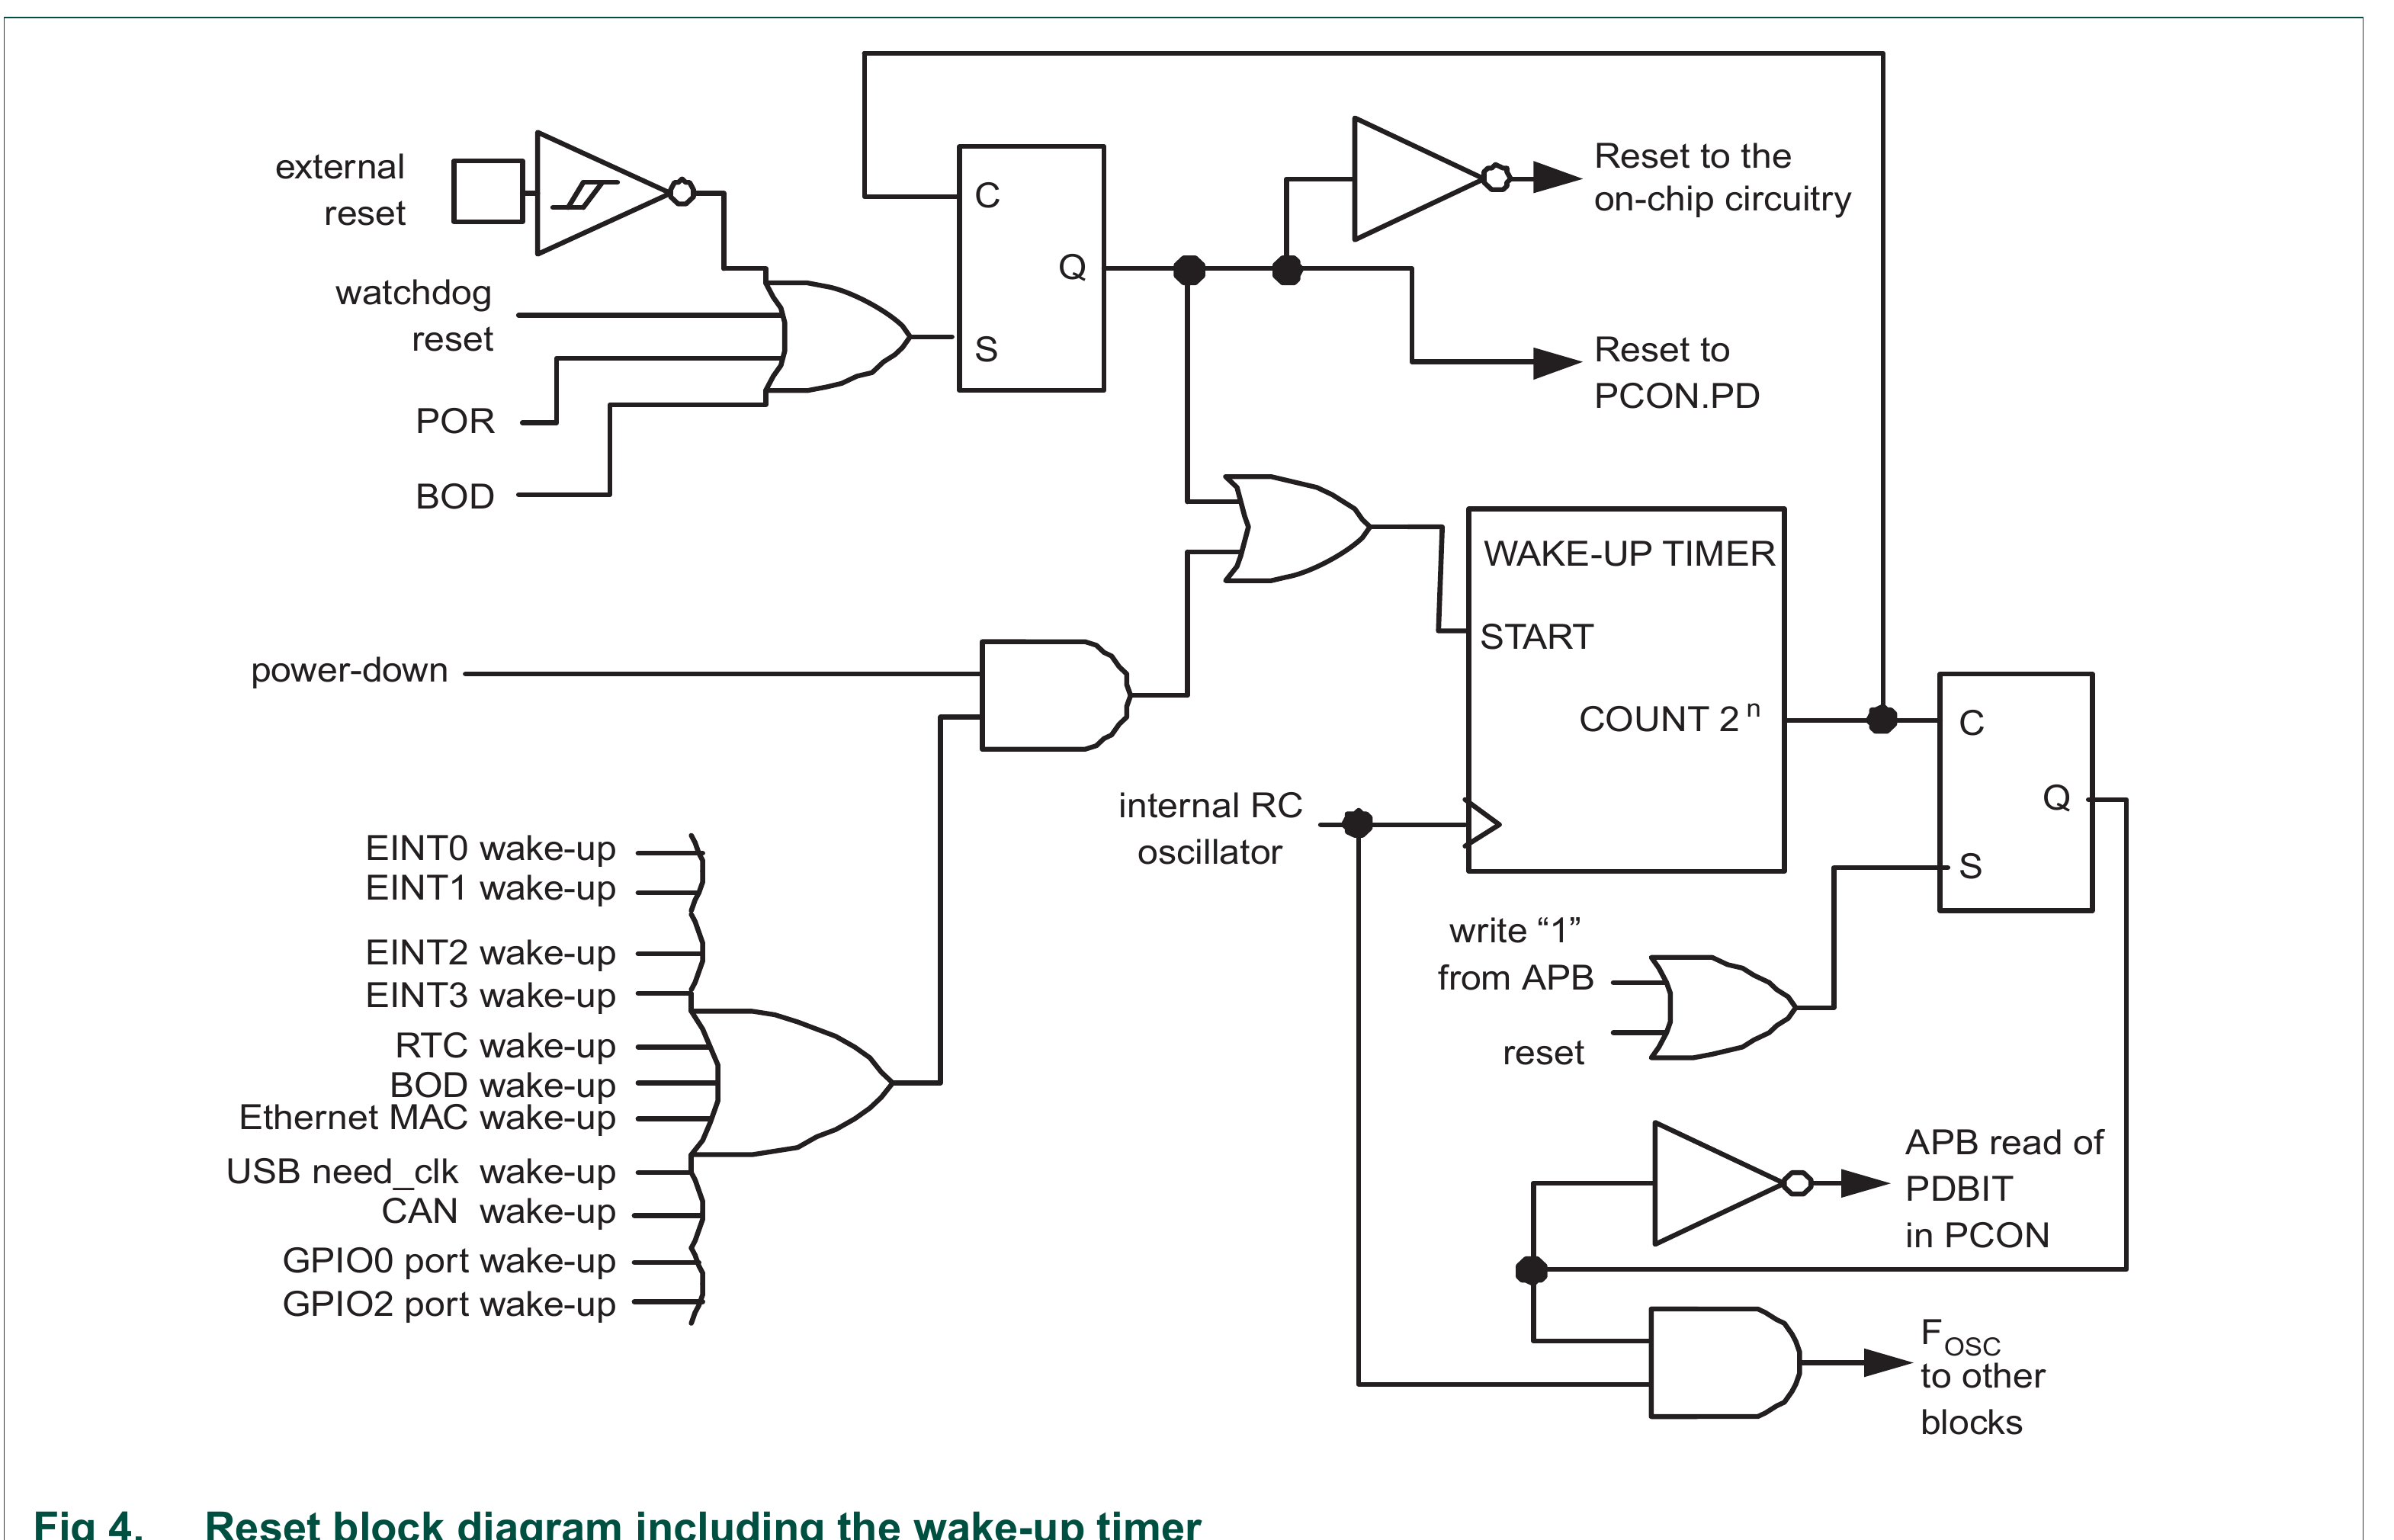
\includegraphics[width=0.96\textwidth]{images/system_control_reset_p19_fig4.png}
  \caption{L\'ogica de reset y \textit{wake-up timer} del bloque System control (Fig 4).}
\end{figure}

\paragraph{Secuencia pr\'actica de arranque}
\begin{enumerate}
  \item Sube la tensi\'on \texttt{VDD(REG)(3V3)} hasta superar el umbral v\'alido de operaci\'on.
  \item Ante una fuente de reset, el primer clock que arranca es el \textit{Internal RC Oscillator} (IRC), que es la fuente de clock por defecto despu\'es de encendido o reset.
  \item Cuando el IRC ya est\'a estable, la l\'ogica interna sincroniza la se\~nal de reset con ese clock.
  \item Desde la liberaci\'on sincronizada del reset corren en paralelo el \textit{IRC wake-up timer} y el temporizador de arranque de la flash.
  \item Cuando la flash ya est\'a lista para ser accedida, comienza la lectura desde memoria y se ejecuta el c\'odigo de arranque en ROM.
  \item Al terminar el \textit{boot code}, el procesador pasa a ejecutar el \textit{user code}. Reci\'en despu\'es, si el firmware lo decide, puede habilitar el oscilador principal y conmutar la fuente de clock en el cap\'itulo 4.
\end{enumerate}

\begin{table}[H]
  \centering
  \small
  \renewcommand{\arraystretch}{1.15}
  \caption{Reset Source Identification register \texttt{RSID} (Table 8)}
  \begin{tabularx}{0.96\textwidth}{|>{\centering\arraybackslash}p{0.08\textwidth}|>{\raggedright\arraybackslash}p{0.14\textwidth}|>{\raggedright\arraybackslash}X|>{\centering\arraybackslash}p{0.12\textwidth}|}
    \hline
    \textbf{Bit} & \textbf{S\'imbolo} & \textbf{Descripci\'on} & \textbf{Reset} \\
    \hline
    \texttt{0} & \texttt{POR} & Se activa con \textit{Power-On Reset}. Tiene prioridad fuerte: al activarse limpia los dem\'as bits, salvo que otra fuente siga presente despu\'es de liberarse el POR. & ver texto \\
    \hline
    \texttt{1} & \texttt{EXTR} & Indica reset por pin \texttt{RESET}. Solo se limpia por software o por POR. & ver texto \\
    \hline
    \texttt{2} & \texttt{WDTR} & Indica reset originado por \textit{Watchdog timeout} con \texttt{WDTRESET=1}. Solo se limpia por software o por POR. & ver texto \\
    \hline
    \texttt{3} & \texttt{BODR} & Indica que \texttt{VDD(REG)(3V3)} cay\'o por debajo del umbral de reset del BOD. Su interpretaci\'on depende de c\'omo cay\'o y se recuper\'o la alimentaci\'on. & ver texto \\
    \hline
    \texttt{31:4} & --- & Reservado. No escribir unos en bits reservados. & NA \\
    \hline
  \end{tabularx}
\end{table}

\paragraph{Nota t\'ecnica}
\texttt{RSID} conviene leerse al inicio del firmware, antes de limpiarlo, si se quiere registrar la causa del reinicio. En particular, \texttt{BODR} solo indica si \texttt{VDD(REG)(3V3)} cay\'o por debajo del umbral BOD cuando ocurre un reset con \texttt{POR=0}.

\subsection{Brown-out detection}
\begin{itemize}
  \item El \textbf{BOD} monitorea \texttt{VDD(REG)(3V3)} con dos umbrales.
  \item Primer nivel: genera una se\~nal hacia el NVIC cuando la tensi\'on cae por debajo del umbral de interrupci\'on (t\'ipicamente \texttt{2.2 V}); si esa interrupci\'on no est\'a habilitada, el evento puede vigilarse leyendo el \textit{Raw Interrupt Status Register}.
  \item Segundo nivel: fuerza reset cuando la tensi\'on cae por debajo del umbral de reset (t\'ipicamente \texttt{1.85 V}).
  \item El objetivo pr\'actico es evitar operaci\'on no confiable y proteger la flash frente a baja tensi\'on.
\end{itemize}

\paragraph{Nota t\'ecnica}
Un \textit{brown-out} transitorio puede sacar al dispositivo de \textit{Power-down} sin dejar un flag de wake-up tan evidente como otros eventos. Si no aparece otra causa latcheada, ese despertar puede atribuirse a BOD.

\subsection{Interrupciones externas \texttt{EINT0..3}}
\begin{itemize}
  \item Cada l\'inea \texttt{EINT} puede configurarse como sensible a \textbf{nivel} o \textbf{flanco}.
  \item En modo nivel, \texttt{EXTPOLAR} elige activo en alto o en bajo.
  \item En modo flanco, \texttt{EXTPOLAR} elige subida o bajada.
  \item Las interrupciones externas tambi\'en pueden actuar como fuente de wake-up desde \textit{Power-down}.
\end{itemize}

\begin{figure}[H]
  \centering
  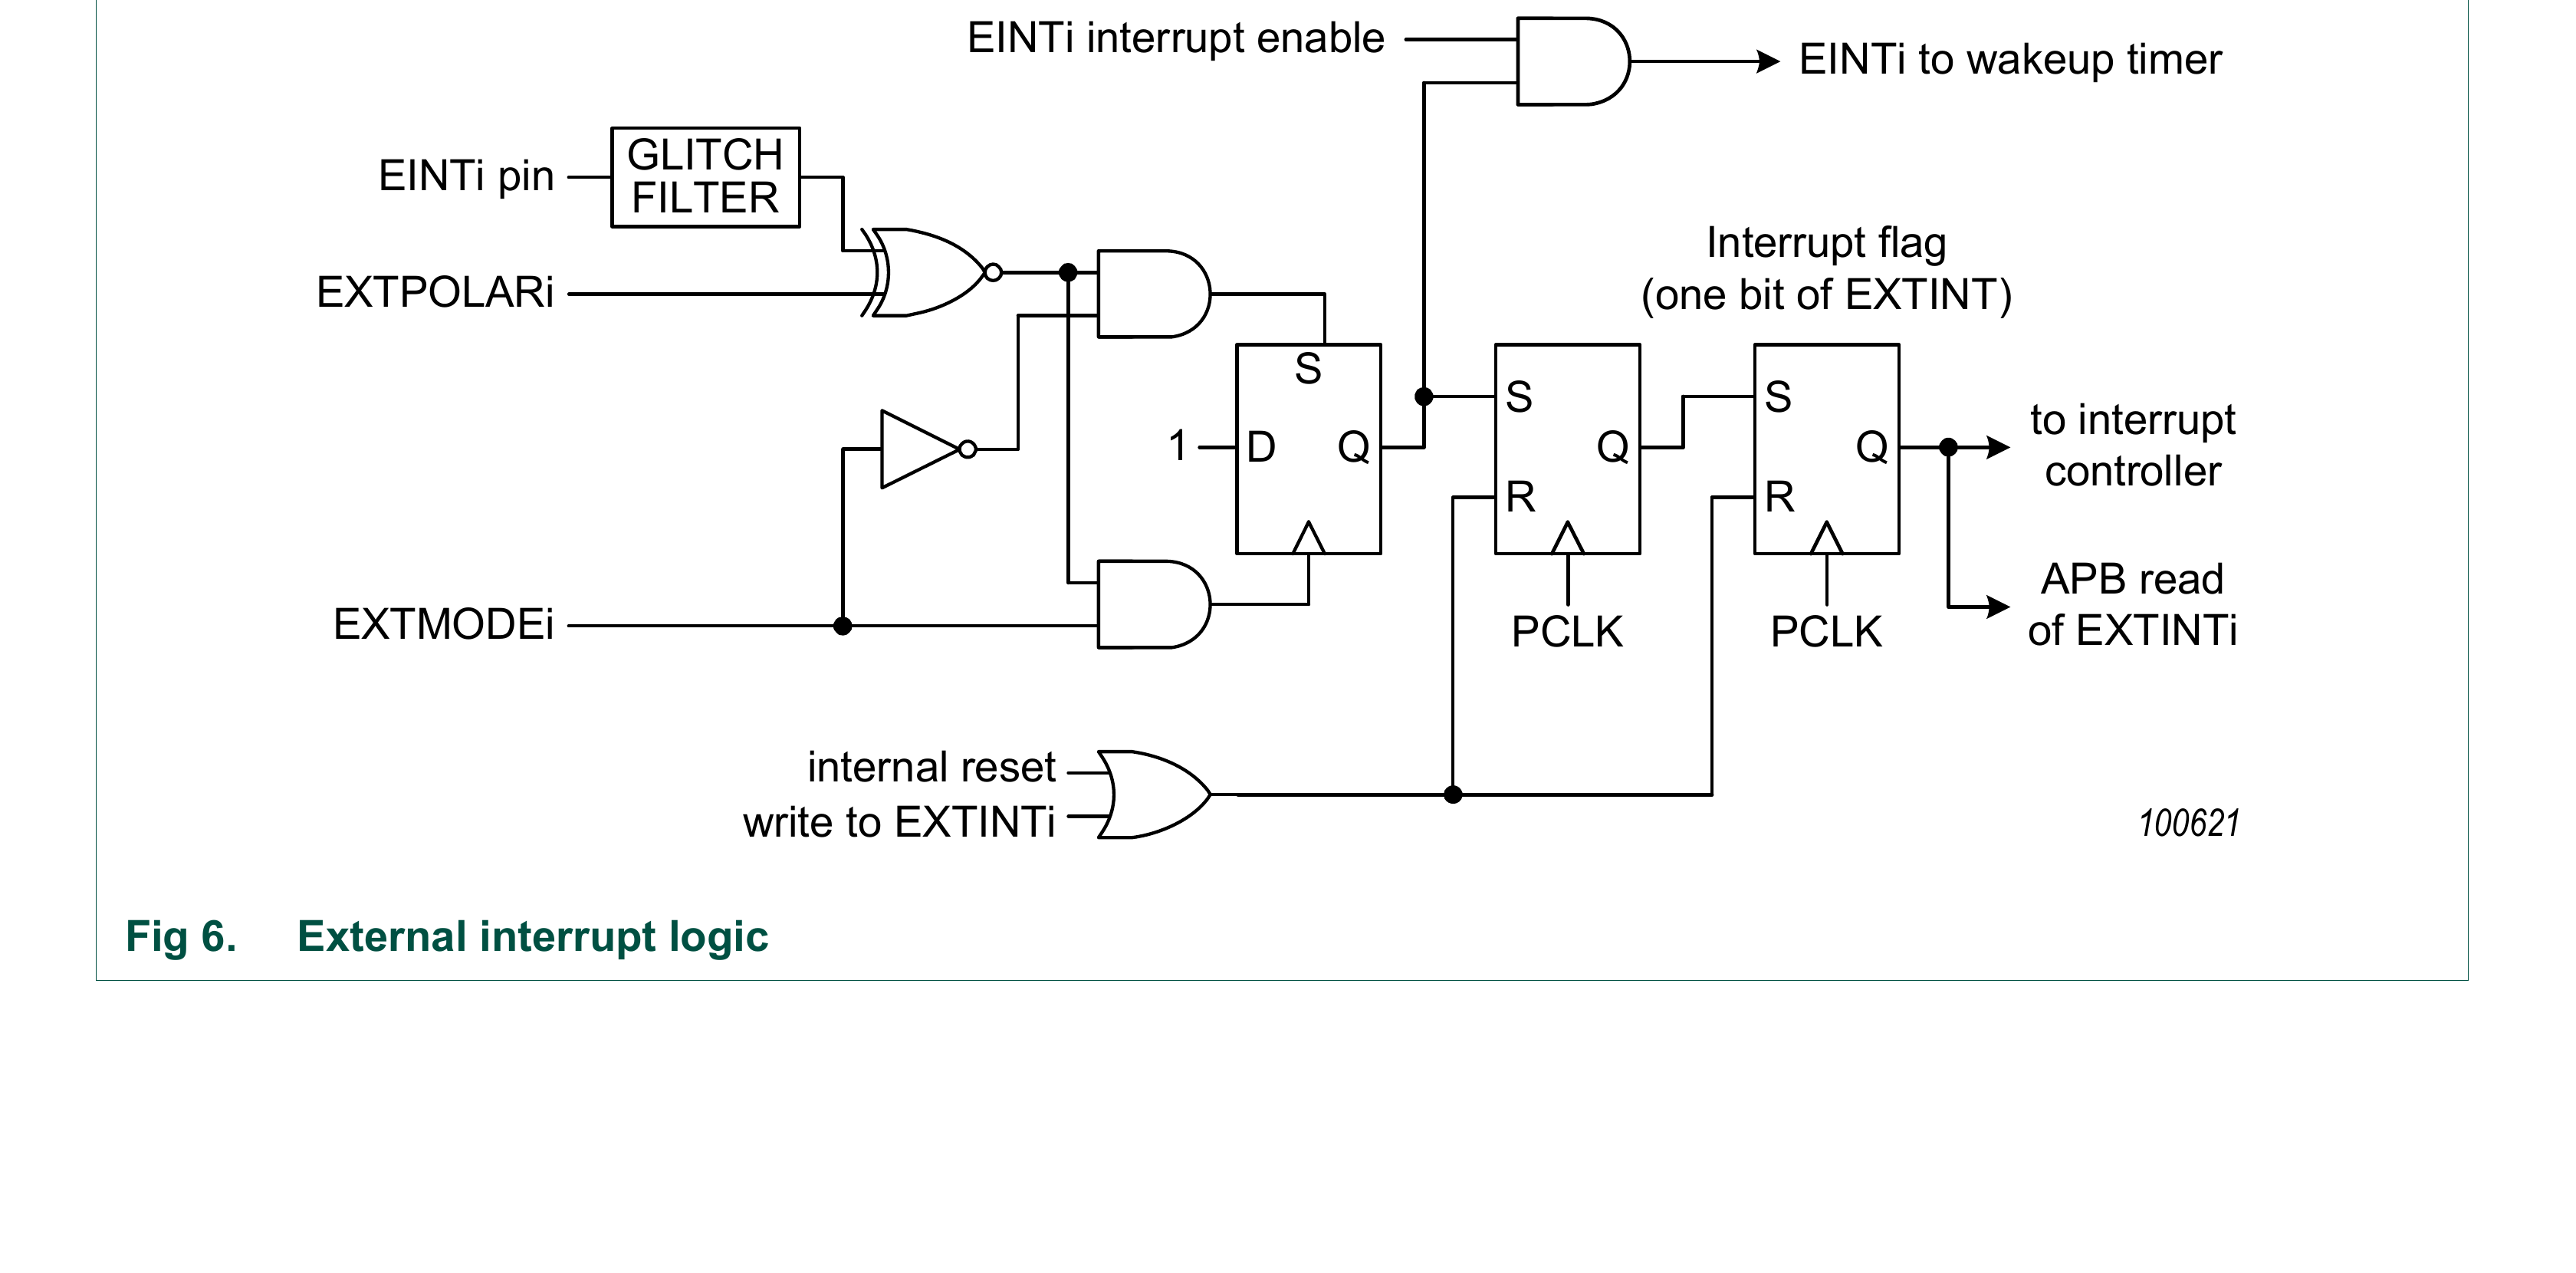
\includegraphics[width=0.96\textwidth]{images/system_control_eint_p23_fig6.png}
  \caption{L\'ogica interna de \texttt{EINTi} y relaci\'on con \texttt{EXTINT}, NVIC y wake-up (Fig 6).}
\end{figure}

\begin{table}[H]
  \centering
  \small
  \renewcommand{\arraystretch}{1.15}
  \caption{External interrupt registers (Table 9)}
  \begin{tabularx}{0.96\textwidth}{|>{\raggedright\arraybackslash}p{0.16\textwidth}|>{\raggedright\arraybackslash}X|>{\centering\arraybackslash}p{0.10\textwidth}|>{\centering\arraybackslash}p{0.10\textwidth}|>{\centering\arraybackslash}p{0.16\textwidth}|}
    \hline
    \textbf{Registro} & \textbf{Funci\'on} & \textbf{Acceso} & \textbf{Reset} & \textbf{Direcci\'on} \\
    \hline
    \texttt{EXTINT} & Flags de interrupci\'on para \texttt{EINT0..3}. & R/W & \texttt{0x00} & \texttt{0x400F C140} \\
    \hline
    \texttt{EXTMODE} & Selecciona sensibilidad por nivel o por flanco. & R/W & \texttt{0x00} & \texttt{0x400F C148} \\
    \hline
    \texttt{EXTPOLAR} & Selecciona nivel alto/bajo o flanco ascendente/descendente. & R/W & \texttt{0x00} & \texttt{0x400F C14C} \\
    \hline
  \end{tabularx}
\end{table}

\begin{table}[H]
  \centering
  \small
  \renewcommand{\arraystretch}{1.15}
  \caption{External Interrupt Flag register \texttt{EXTINT} (Table 10)}
  \begin{tabularx}{0.96\textwidth}{|>{\centering\arraybackslash}p{0.10\textwidth}|>{\raggedright\arraybackslash}p{0.14\textwidth}|>{\raggedright\arraybackslash}X|>{\centering\arraybackslash}p{0.10\textwidth}|}
    \hline
    \textbf{Bit} & \textbf{S\'imbolo} & \textbf{Descripci\'on} & \textbf{Reset} \\
    \hline
    \texttt{0} & \texttt{EINT0} & Flag de evento para \texttt{EINT0}. En modo nivel se mantiene activo mientras el pin permanezca en su estado activo. En modo flanco se activa cuando ocurre el flanco seleccionado. Se limpia escribiendo \texttt{1} en el bit, salvo que el pin siga activo en modo nivel. & \texttt{0} \\
    \hline
    \texttt{1} & \texttt{EINT1} & Igual que el bit anterior, aplicado a \texttt{EINT1}. & \texttt{0} \\
    \hline
    \texttt{2} & \texttt{EINT2} & Igual que el bit anterior, aplicado a \texttt{EINT2}. & \texttt{0} \\
    \hline
    \texttt{3} & \texttt{EINT3} & Igual que el bit anterior, aplicado a \texttt{EINT3}. & \texttt{0} \\
    \hline
    \texttt{31:4} & --- & Reservado. & NA \\
    \hline
  \end{tabularx}
\end{table}

\begin{table}[H]
  \centering
  \small
  \renewcommand{\arraystretch}{1.15}
  \caption{External Interrupt Mode register \texttt{EXTMODE} (Table 11)}
  \begin{tabularx}{0.96\textwidth}{|>{\centering\arraybackslash}p{0.10\textwidth}|>{\raggedright\arraybackslash}p{0.16\textwidth}|>{\raggedright\arraybackslash}X|>{\centering\arraybackslash}p{0.10\textwidth}|}
    \hline
    \textbf{Bit} & \textbf{S\'imbolo} & \textbf{Valor / Descripci\'on} & \textbf{Reset} \\
    \hline
    \texttt{0} & \texttt{EXTMODE0} & \texttt{0}: \texttt{EINT0} sensible a nivel. \texttt{1}: \texttt{EINT0} sensible a flanco. & \texttt{0} \\
    \hline
    \texttt{1} & \texttt{EXTMODE1} & \texttt{0}: \texttt{EINT1} sensible a nivel. \texttt{1}: \texttt{EINT1} sensible a flanco. & \texttt{0} \\
    \hline
    \texttt{2} & \texttt{EXTMODE2} & \texttt{0}: \texttt{EINT2} sensible a nivel. \texttt{1}: \texttt{EINT2} sensible a flanco. & \texttt{0} \\
    \hline
    \texttt{3} & \texttt{EXTMODE3} & \texttt{0}: \texttt{EINT3} sensible a nivel. \texttt{1}: \texttt{EINT3} sensible a flanco. & \texttt{0} \\
    \hline
    \texttt{31:4} & --- & Reservado. & NA \\
    \hline
  \end{tabularx}
\end{table}

\begin{table}[H]
  \centering
  \small
  \renewcommand{\arraystretch}{1.15}
  \caption{External Interrupt Polarity register \texttt{EXTPOLAR} (Table 12)}
  \begin{tabularx}{0.96\textwidth}{|>{\centering\arraybackslash}p{0.10\textwidth}|>{\raggedright\arraybackslash}p{0.16\textwidth}|>{\raggedright\arraybackslash}X|>{\centering\arraybackslash}p{0.10\textwidth}|}
    \hline
    \textbf{Bit} & \textbf{S\'imbolo} & \textbf{Valor / Descripci\'on} & \textbf{Reset} \\
    \hline
    \texttt{0} & \texttt{EXTPOLAR0} & \texttt{0}: \texttt{EINT0} activo en bajo o por flanco descendente. \texttt{1}: \texttt{EINT0} activo en alto o por flanco ascendente. & \texttt{0} \\
    \hline
    \texttt{1} & \texttt{EXTPOLAR1} & \texttt{0}: \texttt{EINT1} activo en bajo o por flanco descendente. \texttt{1}: \texttt{EINT1} activo en alto o por flanco ascendente. & \texttt{0} \\
    \hline
    \texttt{2} & \texttt{EXTPOLAR2} & \texttt{0}: \texttt{EINT2} activo en bajo o por flanco descendente. \texttt{1}: \texttt{EINT2} activo en alto o por flanco ascendente. & \texttt{0} \\
    \hline
    \texttt{3} & \texttt{EXTPOLAR3} & \texttt{0}: \texttt{EINT3} activo en bajo o por flanco descendente. \texttt{1}: \texttt{EINT3} activo en alto o por flanco ascendente. & \texttt{0} \\
    \hline
    \texttt{31:4} & --- & Reservado. & NA \\
    \hline
  \end{tabularx}
\end{table}

\paragraph{Nota t\'ecnica}
Cuando se cambia \texttt{EXTMODE} o \texttt{EXTPOLAR}, el datasheet indica deshabilitar antes la interrupci\'on en el NVIC y escribir \texttt{1} en el bit correspondiente de \texttt{EXTINT} antes de volver a habilitarla. Si no se hace, pueden aparecer interrupciones espurias o fallas al reingresar a \textit{Power-down}.

\subsection{System Controls and Status register}
\begin{itemize}
  \item \texttt{SCS} agrupa bits de control y estado del oscilador principal.
  \item Como el LPC17xx arranca siempre con el \textit{Internal RC Oscillator}, el oscilador principal solo se inicia por pedido expl\'icito de software.
  \item Antes de usarlo como fuente de clock debe seleccionarse el rango de frecuencia y esperarse a que \texttt{OSCSTAT} indique estabilidad.
  \item \texttt{OSCEN=1} solo produce el arranque real del oscilador si la circuiter\'ia externa correcta est\'a conectada a \texttt{XTAL1} y \texttt{XTAL2}.
\end{itemize}

\begin{table}[H]
  \centering
  \small
  \renewcommand{\arraystretch}{1.15}
  \caption{System Controls and Status register \texttt{SCS} (Table 13)}
  \begin{tabularx}{0.96\textwidth}{|>{\centering\arraybackslash}p{0.10\textwidth}|>{\raggedright\arraybackslash}p{0.16\textwidth}|>{\raggedright\arraybackslash}X|>{\centering\arraybackslash}p{0.11\textwidth}|>{\centering\arraybackslash}p{0.10\textwidth}|}
    \hline
    \textbf{Bit} & \textbf{S\'imbolo} & \textbf{Valor / Descripci\'on} & \textbf{Acceso} & \textbf{Reset} \\
    \hline
    \texttt{3:0} & --- & Reservado. & NA & NA \\
    \hline
    \texttt{4} & \texttt{OSCRANGE} & \texttt{0}: rango de \texttt{1 MHz} a \texttt{20 MHz}. \texttt{1}: rango de \texttt{15 MHz} a \texttt{25 MHz}. & R/W & \texttt{0} \\
    \hline
    \texttt{5} & \texttt{OSCEN} & \texttt{0}: oscilador principal deshabilitado. \texttt{1}: oscilador principal habilitado. & R/W & \texttt{0} \\
    \hline
    \texttt{6} & \texttt{OSCSTAT} & \texttt{0}: el oscilador principal todav\'ia no est\'a listo. \texttt{1}: el oscilador principal est\'a estable y listo para usarse. & RO & \texttt{0} \\
    \hline
    \texttt{31:7} & --- & Reservado. & NA & NA \\
    \hline
  \end{tabularx}
\end{table}

\paragraph{Uso pr\'actico}
La secuencia t\'ipica es: configurar \texttt{OSCRANGE}, habilitar \texttt{OSCEN}, esperar \texttt{OSCSTAT=1} y reci\'en despu\'es conmutar la fuente de clock en el cap\'itulo 4.
